\documentclass[hyphens,compress,fleqn]{beamer}
\setbeamercovered{transparent}

\usepackage[utf8]{inputenc}
\usepackage[ngerman]{babel}

\usepackage{array}
\usepackage{tabularx}
\newcolumntype{Z}{>{\raggedright\let\newline\\\arraybackslash}X}

\usepackage{amssymb}
\usepackage{pifont}
\newcommand{\xmark}{\ding{55}}
\usepackage{tikz}
\usepackage{minted}

\useoutertheme[subsection=false]{miniframes}
\usecolortheme{dove}
\usefonttheme[onlysmall]{structurebold}

\addto\captionsngerman{\renewcommand{\figurename}{Abb.}}

\begin{document}
	\title{Dynamische Programmierung (DP)}
	\subtitle{am Beispiel des Wechselgeldproblems}
	\author{Lukas Rost}
	\date{13. Mai 2019}
	
	\begin{frame}[plain]
	\titlepage
	\end{frame}
	
	\section{Das Problem}
	\begin{frame}
		\begin{figure}
			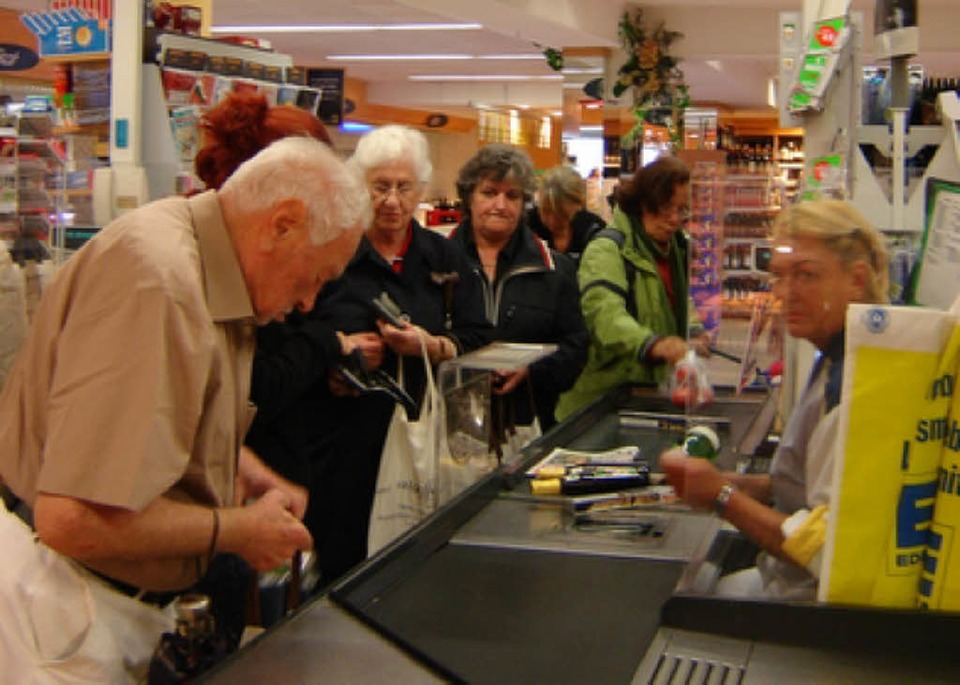
\includegraphics[width=\textwidth]{pics/warteschlange}
		\end{figure}
	\end{frame}

	\begin{frame}{{\footnotesize\insertsectionhead\\}Das Wechselgeldproblem}
		\begin{itemize}[<+->]
			\item Philip steht in der Schlange vor der Kasse im Supermarkt...
			\item ...und möchte den Rentnern vor ihm helfen, das Kleingeld herauszusuchen.
			\item \textbf{Problem:} Rentner brauchen viel Zeit, um eine Münze herauszusuchen.
			\item Philip will Betrag so aufteilen, dass Rentner möglichst wenige Münzen brauchen.
		\end{itemize}
	\end{frame}

	\begin{frame}{{\footnotesize\insertsectionhead\\}Das Wechselgeldproblem}
		\textbf{Formaler:}
		\begin{itemize}[<+->]
			\item Münzwerte: $w = \{w_1,\dots,w_n\}$ mit $w_i \in \mathbb{N}$ und $w_1 = 1$
			\item in Deutschland üblicherweise $w = \{1,2,5,10,\dots\}$
			\item Rechnungssumme: $W$
			\item Anzahl der einzelnen genutzten Münzen: $x = \{x_1,\dots,x_n\}$
			\item Gesamtanzahl der Münzen zu minimieren:
			\begin{align*}
			\min \sum_{j=1}^{n} x_j
			\end{align*}
			\item Bedingung:
			\begin{align*}
			\sum_{j=1}^{n} w_jx_j = W
			\end{align*}
		\end{itemize}
	\end{frame}

	\section{Dynamische Programmierung}
	\begin{frame}{{\footnotesize\insertsectionhead\\}DP als Problemlösungsmethode}
		\begin{itemize}
			\item \textbf{Erfinder:} Richard Bellman (1950er)
			\item Vereinfachen eines komplexen Problems durch Zerlegung in einfache Teilprobleme
			\item ...unter Nutzung von Rekursion
		\end{itemize}
	\end{frame}

	\begin{frame}{{\footnotesize\insertsectionhead\\}Bedingungen für DP}
		\textbf{Optimale Substruktur:}
		\begin{itemize}[<+->]
			\item Lösung eines Optimierungsproblems kann durch Kombination optimaler Teillösungen gefunden werden
			\item \textit{Optimalitätsprinzip von Bellman}
			\item \textit{Beispiel:} Dijkstra
		\end{itemize}
		\vspace*{0.5cm}
		\textbf{Überlappende Subprobleme:}
		\begin{itemize}[<+->]
			\item nur wenige Subprobleme
			\item rekursive Lösung würde die gleichen Subprobleme immer wieder lösen
			\item aber DP löst jedes nur ein Mal!
		\end{itemize}
	\end{frame}

	\begin{frame}{{\footnotesize\insertsectionhead\\}DP-Begriffe}
		\begin{itemize}[<+->]
			\item \textit{DP-Funktion:} $\mathfrak{f}: A \rightarrow B$
			\item \textit{Zustandsraum:} $A$ \\
			Jeder Zustand wird durch Werte der DP-Variablen $x_1,\dots,x_n$ beschrieben
			\item \textit{Werteraum:} $B$
			\item $\mathfrak{f}$ sollte rekursiv berechenbar sein, z.B. Fibonaccizahlen:
			\[
			\mathfrak{f}(n) = \left\{\begin{array}{c c}
			1, & n < 2\\
			\mathfrak{f}(n-1) + \mathfrak{f}(n-2), & n \ge 2
			\end{array}\right.
			\]
			
		\end{itemize}
	\end{frame}

	\begin{frame}{{\footnotesize\insertsectionhead\\}Berechnung der DP-Funktion}
		\begin{itemize}[<+->]
			\item \textbf{Memoization:} Speichern der Ergebnisse von Funktionsaufrufen
			\item geringere Laufzeit, aber dafür höherer Speicherverbrauch
		\end{itemize}
	\end{frame}

	\begin{frame}{{\footnotesize\insertsectionhead\\}Naiv vs. Memoization}
	\begin{columns}
		\begin{column}{.6\textwidth}
			\begin{center}\small
				\begin{figure}
					\begin{tikzpicture}
					\node (f5) [color=red] at (.125,0) {$Fib(5)$};
					\node (f4) [color=red] at (-.5,-1) {$Fib(4)$};
					\node (f3) [color=red] at (-1.75,-2) {$Fib(3)$};
					\node (f2) [color=red] at (-2.9,-3) {$Fib(2)$};
					\node (f1) [color=red] at (-2.9,-4) {$Fib(1)$};
					\node (f0) [color=red] at (-1.75,-4) {$Fib(0)$};
					\node (f12) at (-1.75,-3) {$Fib(1)$};
					\node (f23) at (-.5,-2) {$Fib(2)$};
					\node (f13) at (-.9,-3.5) {$Fib(1)$};
					\node (f03) at (-.155,-4) {$Fib(0)$};
					\node (f35) at (1.25,-1) {$Fib(3)$};
					\node (f25) at (.75,-2) {$Fib(2)$};
					\node (f15) at (.45,-3.5) {$Fib(1)$};
					\node (f05) at (1.2,-3) {$Fib(0)$};
					\node (f16) at (2,-3.5) {$Fib(1)$};
					
					\node (1) [draw, circle] at (0,-5) {$1$};
					
					\path (f25.south) edge [ -> ] (f05.north);
					\path (f25.south) edge [ -> ] (f15.north);
					\path (f35.south) edge [ -> ] (f25.north);
					\path (f35.south) edge [ -> ] (f16.north);
					\path (f5.south) edge [ -> ] (f35.north);
					\path (f4.south) edge [ -> ] (f23.north);
					\path (f23.south) edge [ -> ] (f03.north);
					\path (f23.south) edge [ -> ] (f13.north);
					\path (f5.south) edge [ -> ] (f4.north);
					\path (f4.south) edge [ -> ] (f3.north);
					\path (f3.south) edge [ -> ] (f2.north);
					\path (f3.south) edge [ -> ] (f12.north);
					\path (f2.south) edge [ -> ] (f1.north);
					\path (f2.south) edge [ -> ] (f0.north);
					
					\path (f16.south) edge [ -> ] (1.east);
					\path (f15.south) edge [ -> ] (1.north east);
					\path (f05.south) edge [ -> ] (1.north east);
					\path (f12.south) edge [ -> ] (1.north west);
					\path (f13.south) edge [ -> ] (1.north west);
					\path (f03.south) edge [ -> ] (1.north);
					\path (f1.south) edge [ -> ] (1.west);
					\path (f0.south) edge [ -> ] (1.north west);
					\end{tikzpicture}
					\caption{Naive Lösung: $O(Fib(n))$}
				\end{figure}
			\end{center}
		\end{column}
		\begin{column}{.45\textwidth}
			\begin{center}\small
				\begin{figure}
					\begin{tikzpicture}
					\node (f5) at (0,0) {$Fib(5)$};
					\node (f4) at (0,-1) {$Fib(4)$};
					\node (f3) at (0,-2) {$Fib(3)$};
					\node (f2) at (0,-3) {$Fib(2)$};
					\node (f1) at (1,-4) {$Fib(1)$};
					\node (f0) at (-1,-4) {$Fib(0)$};
					\node (1) [draw, circle] at (0,-5) {$1$};
					
					\path (f5.east) edge [ ->, bend left ] (f4.east);
					\path (f5.east) edge [ ->, bend left ] (f3.east);
					\path (f4.west) edge [ ->, bend right ] (f3.west);
					\path (f4.west) edge [ ->, bend right ] (f2.west);
					\path (f3.east) edge [ ->, bend left ] (f2.east);
					\path (f3.east) edge [ ->, bend left ] (f1.north);
					\path (f2.east) edge [ ->, bend left ] (f1.north);
					\path (f2.west) edge [ ->, bend right ] (f0.north);
					\path (f1.south) edge [ ->, bend left ] (1.east);
					\path (f0.south) edge [ ->, bend right ] (1.west);
					\end{tikzpicture}
					\caption{Schnelle Lösung: $O(n)$}
				\end{figure}
			\end{center}
		\end{column}
	\end{columns}
\end{frame}
\begin{frame}{{\footnotesize\insertsectionhead\\}Bottom-Up vs. Top-Down}
\begin{columns}
\begin{column}{.5\textwidth}
	\begin{center}\small
		\begin{figure}
			\begin{tikzpicture}
			\node (f5) at (0,0) {$Fib(5)$};
			\node (f4) at (0,-1) {$Fib(4)$};
			\node (f3) at (0,-2) {$Fib(3)$};
			\node (f2) at (0,-3) {$Fib(2)$};
			\node (f1) at (1,-4) {$Fib(1)$};
			\node (f0) at (-1,-4) {$Fib(0)$};
			\node (1) [draw, circle] at (0,-5) {$1$};
			
			\path (f5.east) edge [ ->, bend left ] (f4.east);
			\path (f5.east) edge [ ->, bend left ] (f3.east);
			\path (f4.west) edge [ ->, bend right ] (f3.west);
			\path (f4.west) edge [ ->, bend right ] (f2.west);
			\path (f3.east) edge [ ->, bend left ] (f2.east);
			\path (f3.east) edge [ ->, bend left ] (f1.north);
			\path (f2.east) edge [ ->, bend left ] (f1.north);
			\path (f2.west) edge [ ->, bend right ] (f0.north);
			\path (f1.south) edge [ ->, bend left ] (1.east);
			\path (f0.south) edge [ ->, bend right ] (1.west);
			\end{tikzpicture}
			\caption{„Top-Down“ DP}
		\end{figure}
	\end{center}
\end{column}
\begin{column}{.5\textwidth}
	\begin{center}\small
		\begin{figure}
			\begin{tikzpicture}
			\node (f5) at (0,0) {$Fib(5)$};
			\node (f4) at (0,-1) {$Fib(4)$};
			\node (f3) at (0,-2) {$Fib(3)$};
			\node (f2) at (0,-3) {$Fib(2)$};
			\node (f1) at (1,-4) {$Fib(1)$};
			\node (f0) at (-1,-4) {$Fib(0)$};
			\node (1) [draw, circle] at (0,-5) {$1$};
			
			\path (f5.east) edge [ <-, bend left ] (f4.east);
			\path (f5.east) edge [ <-, bend left ] (f3.east);
			\path (f4.west) edge [ <-, bend right ] (f3.west);
			\path (f4.west) edge [ <-, bend right ] (f2.west);
			\path (f3.east) edge [ <-, bend left ] (f2.east);
			\path (f3.east) edge [ <-, bend left ] (f1.north);
			\path (f2.east) edge [ <-, bend left ] (f1.north);
			\path (f2.west) edge [ <-, bend right ] (f0.north);
			\path (f1.south) edge [ <-, bend left ] (1.east);
			\path (f0.south) edge [ <-, bend right ] (1.west);
			\end{tikzpicture}
			\caption{„Bottom-Up“ DP}
		\end{figure}
	\end{center}
\end{column}
\end{columns}
\end{frame}


	\section{Die Lösung}
	\begin{frame}{{\footnotesize\insertsectionhead\\}Greedy-Ansatz}
	\begin{itemize}[<+->]
		\item einfach den größten Münzwert nehmen, der den verbleibenden Betrag nicht übersteigt
		\item \textbf{Problem:} funktioniert nur für \textit{kanonische Münzsysteme} wie in Deutschland oder USA
		\item Was ist, wenn Philip in \textit{Templonia} lebt?
		\item Dort gibt es nur 1, 3 und 4 templonische Säulen als Münzwerte!
	\end{itemize}
	\end{frame}

	\begin{frame}{{\footnotesize\insertsectionhead\\}DP-Lösung}
	\begin{itemize}[<+->]
		\item \textit{DP-Variable:} $x$ (zu erreichende Summe)
		\item \textit{DP-Wert:} $\mathfrak{f}(x)$ (minimale Anzahl benötigter Münzen)
		\item \textit{DP-Funktion:}\begin{align*}
		& \mathfrak{f}(x) =
		\begin{cases}
		\infty & x < 0 \\
		0 & x = 0 \\
		\min_{i = 1}^{n} \mathfrak{f}(x-w_i) + 1 & x > 0
		\end{cases}
		\end{align*}
		\item Idee: Möglichkeiten für erste Münze durchprobieren und beste wählen
		\item gesuchtes Ergebnis: $\mathfrak{f}(W)$
		\item läuft durch DP in $\mathcal{O}(n\cdot W)$
	\end{itemize}
	\end{frame}

	\begin{frame}{{\footnotesize\insertsectionhead\\}DP-Lösung}
	\begin{itemize}[<+->]
		\item Wie erhält man daraus die eigentliche Lösung (Anzahl der einzelnen Münzen)?
		\item ganz einfach: für jeden Wert die erste benötigte Münze speichern
		\item \dots und dann backtracen
	\end{itemize}
	\end{frame}

	\begin{frame}[fragile]{{\footnotesize\insertsectionhead\\}Implementierung}
	\begin{minted}[frame=single]{cpp}
value[0] = 0;
for(int j = 1; j <= n; j++){
	value[j] = INF;
	for(auto c: coins){
	  if(j-c >= 0 && value[j-c]+1 < value[j]){
		  value[j] = value[j-c]+1;
		  first[j] = c;
	  }
	}
}
	\end{minted}
	\end{frame}

	\begin{frame}[plain]{Bildquellen}
		\begin{itemize}
			\item \url{http://ais.fudder.de/piece/07/12/b7/78/118667128-w-960.jpg}
			\item Vorträge und Aufgaben des IOI-Trainings
		\end{itemize}
	\end{frame}

\end{document}